% A LaTeX template for MSc Thesis submissions to 
% Politecnico di Milano (PoliMi) - School of Industrial and Information Engineering
%
% S. Bonetti, A. Gruttadauria, G. Mescolini, A. Zingaro
% e-mail: template-tesi-ingind@polimi.it
%
% Last Revision: October 2021
%
% Copyright 2021 Politecnico di Milano, Italy. NC-BY

\documentclass{Configuration_Files/PoliMi3i_thesis}

%------------------------------------------------------------------------------
%	REQUIRED PACKAGES AND  CONFIGURATIONS
%------------------------------------------------------------------------------

% CONFIGURATIONS
\usepackage{parskip} % For paragraph layout
\usepackage{setspace} % For using single or double spacing
\usepackage{emptypage} % To insert empty pages
\usepackage{multicol} % To write in multiple columns (executive summary)
\setlength\columnsep{15pt} % Column separation in executive summary
\setlength\parindent{0pt} % Indentation
\raggedbottom  

% PACKAGES FOR TITLES
\usepackage{titlesec}
% \titlespacing{\section}{left spacing}{before spacing}{after spacing}
\titlespacing{\section}{0pt}{3.3ex}{2ex}
\titlespacing{\subsection}{0pt}{3.3ex}{1.65ex}
\titlespacing{\subsubsection}{0pt}{3.3ex}{1ex}
\usepackage{color}

% PACKAGES FOR LANGUAGE AND FONT
\usepackage[english]{babel} % The document is in English  
\usepackage[utf8]{inputenc} % UTF8 encoding
\usepackage[T1]{fontenc} % Font encoding
\usepackage[11pt]{moresize} % Big fonts

% PACKAGES FOR IMAGES
\usepackage{graphicx}
\usepackage{transparent} % Enables transparent images
\usepackage{eso-pic} % For the background picture on the title page
\usepackage{subfig} % Numbered and caption subfigures using \subfloat.
\usepackage{tikz} % A package for high-quality hand-made figures.
\usetikzlibrary{}
\graphicspath{{./Images/}} % Directory of the images
\usepackage{caption} % Coloured captions
\usepackage{xcolor} % Coloured captions
\usepackage{amsthm,thmtools,xcolor} % Coloured "Theorem"
\usepackage{float}

% STANDARD MATH PACKAGES
\usepackage{amsmath}
\usepackage{amsthm}
\usepackage{amssymb}
\usepackage{amsfonts}
\usepackage{bm}
\usepackage[overload]{empheq} % For braced-style systems of equations.
\usepackage{fix-cm} % To override original LaTeX restrictions on sizes

% PACKAGES FOR TABLES
\usepackage{tabularx}
\usepackage{longtable} % Tables that can span several pages
\usepackage{colortbl}

% PACKAGES FOR ALGORITHMS (PSEUDO-CODE)
\usepackage{algorithm}
\usepackage{algorithmic}

% PACKAGES FOR REFERENCES & BIBLIOGRAPHY
\usepackage[colorlinks=true,linkcolor=black,anchorcolor=black,citecolor=black,filecolor=black,menucolor=black,runcolor=black,urlcolor=black]{hyperref} % Adds clickable links at references
\usepackage{cleveref}
\usepackage[square, numbers, sort&compress]{natbib} % Square brackets, citing references with numbers, citations sorted by appearance in the text and compressed
\bibliographystyle{abbrvnat} % You may use a different style adapted to your field

% OTHER PACKAGES
\usepackage{pdfpages} % To include a pdf file
\usepackage{afterpage}
\usepackage{lipsum} % DUMMY PACKAGE
\usepackage{fancyhdr} % For the headers
\fancyhf{}

\usepackage{graphicx}
\usepackage{tocloft}  
\usepackage{titling}  
\usepackage{booktabs} 
\usepackage{tabularx}  
\usepackage{geometry} 
\usepackage{longtable}
\usepackage{multirow}
\usepackage{todonotes}
\usepackage{listings}
\usepackage{xcolor}
\usepackage{amsmath} 

% Define colors for custom Alloy highlighting
\definecolor{commentgreen}{rgb}{0,0.6,0}
\definecolor{keywordblue}{rgb}{0.13,0.13,1}
\definecolor{stringred}{rgb}{0.8,0,0}
\definecolor{numberpurple}{rgb}{0.58,0,0.83}

% Define Alloy language syntax highlighting
\lstdefinelanguage{Alloy}{
    keywords={sig, extends, fact, pred, fun, run, assert, check, some, all, no, one, lone, abstract, disj, module, open, set},
    keywordstyle=\color{keywordblue}\bfseries,
    comment=[l]{//},              % comment style
    commentstyle=\color{commentgreen},
    stringstyle=\color{stringred},
    morestring=[b]",              % strings are in quotes
    sensitive=true,               % case sensitive
    morekeywords={in, and, or, not, implies, iff}, % Alloy-specific keywords
    morecomment=[s]{/*}{*/},      % block comment style
    literate={0}{{\textcolor{numberpurple}{0}}}{1}%
             {1}{{\textcolor{numberpurple}{1}}}{1}%
             {2}{{\textcolor{numberpurple}{2}}}{1}%
             {3}{{\textcolor{numberpurple}{3}}}{1}%
             {4}{{\textcolor{numberpurple}{4}}}{1}%
             {5}{{\textcolor{numberpurple}{5}}}{1}%
             {6}{{\textcolor{numberpurple}{6}}}{1}%
             {7}{{\textcolor{numberpurple}{7}}}{1}%
             {8}{{\textcolor{numberpurple}{8}}}{1}%
             {9}{{\textcolor{numberpurple}{9}}}{1}%
}

\lstset{
    language=Alloy,
    basicstyle=\ttfamily\footnotesize,
    numbers=left,
    numberstyle=\tiny\color{gray},
    stepnumber=1,
    breaklines=true,
    showstringspaces=false,
    frame=single,
    caption=Alloy Example,
    label=code:alloy_example,
}

\setlength{\cftbeforesecskip}{10pt}


% Input of configuration file. Do not change config.tex file unless you really know what you are doing. 
% Define blue color typical of polimi
\definecolor{bluepoli}{cmyk}{0.4,0.1,0,0.4}

% Custom theorem environments
\declaretheoremstyle[
  headfont=\color{bluepoli}\normalfont\bfseries,
  bodyfont=\color{black}\normalfont\itshape,
]{colored}

% Set-up caption colors
\captionsetup[figure]{labelfont={color=bluepoli}} % Set colour of the captions
\captionsetup[table]{labelfont={color=bluepoli}} % Set colour of the captions
\captionsetup[algorithm]{labelfont={color=bluepoli}} % Set colour of the captions

\theoremstyle{colored}
\newtheorem{theorem}{Theorem}[chapter]
\newtheorem{proposition}{Proposition}[chapter]

% Enhances the features of the standard "table" and "tabular" environments.
\newcommand\T{\rule{0pt}{2.6ex}}
\newcommand\B{\rule[-1.2ex]{0pt}{0pt}}

% Pseudo-code algorithm descriptions.
\newcounter{algsubstate}
\renewcommand{\thealgsubstate}{\alph{algsubstate}}
\newenvironment{algsubstates}
  {\setcounter{algsubstate}{0}%
   \renewcommand{\STATE}{%
     \stepcounter{algsubstate}%
     \Statex {\small\thealgsubstate:}\space}}
  {}

% New font size
\newcommand\numfontsize{\@setfontsize\Huge{200}{60}}

% Title format: chapter
\titleformat{\chapter}[hang]{
\fontsize{50}{20}\selectfont\bfseries\filright}{\textcolor{bluepoli} \thechapter\hsp\hspace{2mm}\textcolor{bluepoli}{|   }\hsp}{0pt}{\huge\bfseries \textcolor{bluepoli}
}

% Title format: section
\titleformat{\section}
{\color{bluepoli}\normalfont\Large\bfseries}
{\color{bluepoli}\thesection.}{1em}{}

% Title format: subsection
\titleformat{\subsection}
{\color{bluepoli}\normalfont\large\bfseries}
{\color{bluepoli}\thesubsection.}{1em}{}

% Title format: subsubsection
\titleformat{\subsubsection}
{\color{bluepoli}\normalfont\large\bfseries}
{\color{bluepoli}\thesubsubsection.}{1em}{}

% Shortening for setting no horizontal-spacing
\newcommand{\hsp}{\hspace{0pt}}

\makeatletter
% Renewcommand: cleardoublepage including the background pic
\renewcommand*\cleardoublepage{%
  \clearpage\if@twoside\ifodd\c@page\else
  \null
  \AddToShipoutPicture*{\BackgroundPic}
  \thispagestyle{empty}%
  \newpage
  \if@twocolumn\hbox{}\newpage\fi\fi\fi}
\makeatother

%For correctly numbering algorithms
\numberwithin{algorithm}{chapter}


%----------------------------------------------------------------------------
%	NEW COMMANDS DEFINED
%----------------------------------------------------------------------------

% EXAMPLES OF NEW COMMANDS
\newcommand{\bea}{\begin{eqnarray}} % Shortcut for equation arrays
\newcommand{\eea}{\end{eqnarray}}
\newcommand{\e}[1]{\times 10^{#1}}  % Powers of 10 notation

%----------------------------------------------------------------------------
%	ADD YOUR PACKAGES (be careful of package interaction)
%----------------------------------------------------------------------------

%----------------------------------------------------------------------------
%	ADD YOUR DEFINITIONS AND COMMANDS (be careful of existing commands)
%----------------------------------------------------------------------------

%----------------------------------------------------------------------------
%	BEGIN OF YOUR DOCUMENT
%----------------------------------------------------------------------------

\begin{document}

\fancypagestyle{plain}{%
\fancyhf{} % Clear all header and footer fields
\fancyhead[RO,RE]{\thepage} %RO=right odd, RE=right even
\renewcommand{\headrulewidth}{0pt}
\renewcommand{\footrulewidth}{0pt}}

%----------------------------------------------------------------------------
%	TITLE PAGE
%----------------------------------------------------------------------------

\pagestyle{empty} % No page numbers
\frontmatter % Use roman page numbering style (i, ii, iii, iv...) for the preamble pages

\puttitle{
    title=Requirement Analysis and Specification, % Title of the thesis
    nameA=Giovanni Vaccarino, % Author Name and Surname
    nameB=Vittorio Palladino, % Author Name and Surname
    nameC=Nicolò Vacis, % Author Name and Surname
    course=Computer Science and Engineering, % Study Programme (in Italian)
    academicyear={2024{-}25},  % Academic Year
} % These info will be put into your Title page 

%----------------------------------------------------------------------------
%	LIST OF CONTENTS/FIGURES/TABLES/SYMBOLS
%----------------------------------------------------------------------------

% TABLE OF CONTENTS
\thispagestyle{empty}
\tableofcontents % Table of contents 
\thispagestyle{empty}
\cleardoublepage

%-------------------------------------------------------------------------
%	THESIS MAIN TEXT
%-------------------------------------------------------------------------
% In the main text of your thesis you can write the chapters in two different ways:
%
%(1) As presented in this template you can write:
%    \chapter{Title of the chapter}
%    *body of the chapter*
%
%(2) You can write your chapter in a separated .tex file and then include it in the main file with the following command:
%    \chapter{Title of the chapter}
%    \input{chapter_file.tex}
%
% Especially for long thesis, we recommend you the second option.

\addtocontents{toc}{\vspace{2em}} % Add a gap in the Contents, for aesthetics
\mainmatter % Begin numeric (1,2,3...) page numbering

% --------------------------------------------------------------------------
% NUMBERED CHAPTERS % Regular chapters following
% --------------------------------------------------------------------------

\chapter{Introduction}
\section{Scope}

The S\&C platform is a web-based solution intended to support:
\begin{itemize}
    \item \textbf{Students} in finding internships suited to their skills and aspirations, allowing them to submit CVs and receive tailored recommendations.
    \item \textbf{Companies} in listing internship opportunities and identifying candidates based on skills and profiles.
    \item \textbf{Universities} in overseeing internships, tracking progress, addressing complaints, and ensuring the quality of internships.
\end{itemize}
The platform enables interaction among these groups, handling tasks like matching candidates with internships, interview scheduling, feedback collection, and assessing internship effectiveness. The platform is built to scale across universities, supporting thousands of users.

\section{Definitions, Acronyms, Abbreviations}

\subsection{Definitions}
\begin{itemize}
    \item \textbf{Slug}: A human-readable and URL-friendly string (typically lowercase ASCII characters) that uniquely identifies a specific resource. It is commonly used in URLs but may also serve as an identifier for resources, like internship listings or profiles, within the S\&C platform.
    \item \textbf{S\&C Repository Slug}: A slug in the format `<repository owner>/<repository name>` that uniquely identifies a project repository on the S\&C platform or external GitHub repositories associated with student or company projects.
\end{itemize}

\subsection{Acronyms}
\begin{itemize}
    \item \textbf{S\&C}: Students\&Companies platform
    \item \textbf{API}: Application Programming Interface
    \item \textbf{CV}: Curriculum Vitae
    \item \textbf{GDPR}: General Data Protection Regulation
    \item \textbf{GH}: GitHub
    \item \textbf{SSO}: Single Sign-On
    \item \textbf{UUID}: Universal Unique Identifier
    \item \textbf{DB}: Database
    \item \textbf{DBMS}: Database Management System
    \item \textbf{RPC}: Remote Procedure Call
    \item \textbf{REST}: Representational State Transfer
    \item \textbf{SPA}: Single Page Application
    \item \textbf{CDN}: Content Delivery Network
\end{itemize}

\subsection{Abbreviations}
\begin{itemize}
    \item \textbf{e.g.}: For example
    \item \textbf{repo}: Repository
    \item \textbf{ID}: Identifier
\end{itemize}

\section{Revision History}
\begin{table}[h!]
\centering
\begin{tabular}{|c|c|l|}
\hline
\textbf{Version} & \textbf{Date} & \textbf{Description} \\ \hline
1.0 & January 7, 2024 & Initial release \\ \hline
\end{tabular}
\end{table}


\section{Reference Documents}
\begin{itemize}
    \item Specification document: "Assignment RDD AY 2023-2024"
    \item UML official specification: \url{https://www.omg.org/spec/UML/}
    \item Requirements Analysis and Specification Document: "RASD"
\end{itemize}

\section{Document Structure}
The document is organized into the following sections:
\begin{itemize}
    \item \textbf{Section 1: Introduction} - Provides an overview of the problem and the system's scope. It also includes definitions, acronyms, abbreviations, and a revision history to track document versions and modifications.
    \item \textbf{Section 2: Architectural Design} - Describes the system architecture, starting with a high-level overview of design choices, followed by detailed component and deployment views, including server, client, and data components (DB schemas). This section also presents sequence diagrams to illustrate the system’s runtime view and includes information on component interfaces, design styles, and architectural patterns.
    \item \textbf{Section 3: User Interface Design} - Outlines the design of the user interface, providing an overview of the platform’s visual layout and user interactions.
    \item \textbf{Section 4: Requirements Traceability} - Maps the requirements from the RASD to corresponding design elements in this document.
    \item \textbf{Section 5: Implementation, Integration, and Test Plan} - Details the implementation order of the system’s subcomponents, integration steps, and testing procedures to ensure system reliability.
\end{itemize}



\chapter{Overall Description}
\section{Product Perspective}
\subsection{Domain's class diagram (simplified)}
\begin{figure}[!ht]
    \centering
    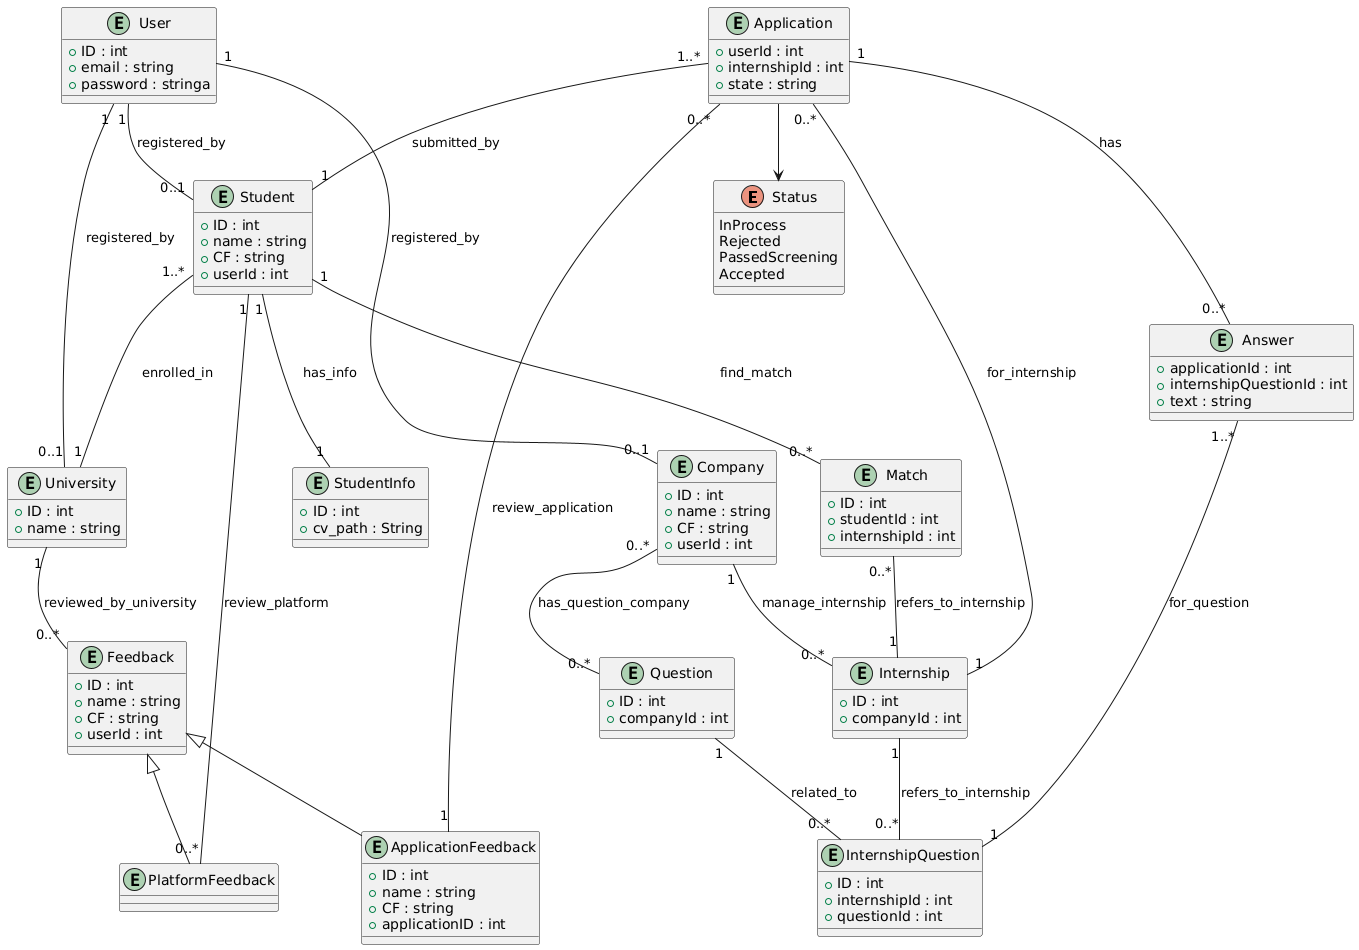
\includegraphics[scale=0.35]{Images/ImagesRASD/class_diagram.png}
    \caption{Class diagram}
\end{figure}

\newpage
\subsection{Scenarios and state diagrams}
The following scenarios illustrate interactions between students, companies, and the S\&C platform.
In order to explain the behavior of some scenarios, we decide to adopt the use of BPMN instead of UML state diagrams, because better describes the exchange of information and messages between the actors (Look for it in the references).

\begin{itemize}
    \item \textbf{Scenario 1: Student registers and uploads CV.}  \\
    Maria, a third-year university student, is looking for internship opportunities to gain practical experience. She discovers the S\&C platform, which connects students with relevant internships. To get started, she navigates to the registration page of the S\&C platform. Maria provides her personal information, including her name, email, university, and area of study, and sets up a secure password. The platform verifies her email through a confirmation link sent to her inbox. After verifying, Maria is successfully registered and directed to her dashboard. Here, she completes her profile by specifying her skills, interests, and career aspirations, and uploads her CV to showcase her academic background, work experience, and skills. The system securely stores this information and uses it to generate internship recommendations tailored to Maria’s profile. She is informed that she can update her profile over time to refine these recommendations.

    \begin{figure}[!ht]
    \centering
    \includegraphics[scale=0.30]{Images/ImagesRASD/scenario_1.png}
    \caption{BPMN diagram scenario 1}
    \end{figure}

    \item \textbf{Scenario 2: Company registers.} \\
    CodeWorks, a tech company specializing in front-end development, decides to utilize the S\&C platform to find potential interns. The HR manager at CodeWorks begins by registering the company on the platform. They navigate to the company registration page, where they provide essential details such as the company name, industry, location, and a contact email, setting up a password for secure access. After submitting the information, a verification email is sent to the contact email provided. The HR manager completes the verification process by clicking the link, activating the company account on the platform. Once logged in, the HR manager is directed to the company dashboard, where they can create a profile for CodeWorks, detailing the company's values, areas of expertise, and the potential for future internship opportunities. The profile is saved and made visible to students interested in relevant industries, allowing CodeWorks to engage student attention even before posting a specific internship.

    \item \textbf{Scenario 3: Company posts a new internship.} \\
    After creating a profile, CodeWorks is ready to post an internship position. The HR manager logs into the S\&C platform and selects the option to post a new internship. They complete fields for the job title, required skills, internship duration, and benefits, such as mentorship and training opportunities. After submitting the internship details, the listing becomes visible to students whose profiles match the job criteria. The platform also flags the listing for students seeking roles in tech, ensuring greater exposure to qualified candidates. 

    \item \textbf{Scenario 4: Student receives internship recommendations.}  \\
    After setting up her profile, Maria begins exploring opportunities. Based on her profile, the S\&C platform’s recommendation engine suggests internships that align with her background. She receives a curated list of potential matches, including details like the position title, required skills, project descriptions, and company information. As Maria browses, she finds an internship at CodeWorks and decides to apply, with the platform offering further details on the company culture, job role expectations, and deadlines.
    
    \item \textbf{Scenario 5: Company reviews applications and selects candidates for interviews.} \\ 
    CodeWorks reviews submissions for the internship. The HR team logs in to the S\&C platform and accesses a list of applicants, including Maria, with CVs and profile details. They can filter applicants by skill level and background. After review, CodeWorks shortlists Maria and other candidates for interviews. The S\&C platform assists in scheduling and notifies Maria of her interview, providing her with preparation tips and interview details.

    \begin{figure}[!ht]
    \centering
    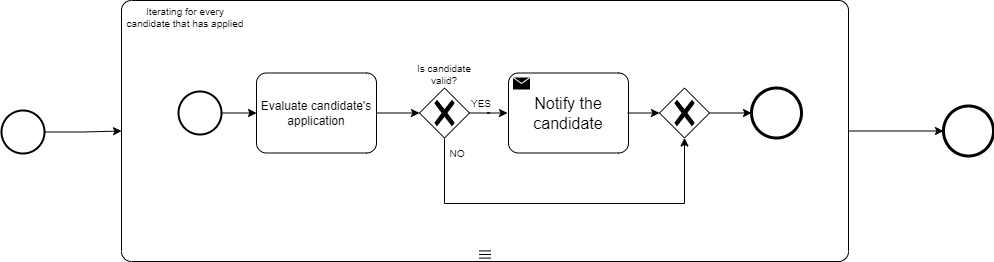
\includegraphics[scale=0.30]{Images/ImagesRASD/scenario_5.png}
    \caption{BPMN diagram scenario 5}
    \end{figure}

    \item \textbf{Scenario 6: University monitors student internship progress.} \\
    Maria’s university requires students to complete an internship and uses the S\&C platform to monitor student progress. Once Maria secures the internship at CodeWorks, her university’s coordinator views her status, including the start date, role, and completion date. A dashboard allows the coordinator to track Maria’s feedback and address any concerns. If Maria or CodeWorks reports issues, the coordinator is notified, enabling them to assist in resolving challenges like scheduling conflicts or misaligned expectations.

    \item \textbf{Scenario 7: Student submits feedback and receives certificate upon internship completion.}  \\
    After completing her internship, Maria is prompted to submit feedback on her experience at CodeWorks. She completes a form rating aspects such as mentorship, skill development, and overall satisfaction. The feedback is anonymized and shared with CodeWorks for future improvement. Upon submission, the platform generates an internship completion certificate for Maria, which she can download from her profile. This certificate and feedback contribute to analyses that enhance future recommendations for students.
\end{itemize}

\newpage

\section{Product Functions}

The Students\&Companies (S\&C) platform serves as an intermediary between students seeking internship opportunities and companies offering them. The primary goal of the platform is to facilitate a streamlined and efficient matchmaking process, providing both students and companies with a robust set of functionalities tailored to their unique needs. Below, the most important requirements of the system are outlined, focusing on core functions that enable users to interact, apply, and manage internships effectively.
\subsection{G1: Student Registration and Profile Management}
\begin{itemize}
    \item R1: Dashboard with recommended internships — The system shall provide students with a personalized dashboard displaying internships tailored to their profile, along with application statuses and feedback.
    \item R2: Profile creation and editing — Students must be able to create a profile by entering key details such as education, skills, and career interests, and be allowed to update this information to refine recommendations.
    \item R3: Search tool with filtering options — The platform shall offer students a search tool with filters for location, field of study, and skills to find suitable internships.
    \item R4: Step-by-step application guidance — The system shall guide students through the application process with a wizard that displays deadlines and tracks progress.
    \item R13: Detailed profile management with CV upload — The platform shall support a detailed profile structure where students can upload and manage their CV to showcase their qualifications to potential employers.
\end{itemize}

\subsection{G2: Company Registration and Internship Posting}
\begin{itemize}
    \item R5: Internship posting management — The system shall allow companies to create, update, and manage internship listings with details such as job title, required skills, duration, and benefits.
    \item R6: Company dashboard for reviewing applications — Companies should have a dashboard where they can view applications, assess candidate profiles, and filter applicants based on skills and qualifications.
    \item R14: Set deadlines and manage postings — Companies must be able to set deadlines for applications and update or close postings as positions are filled or requirements change.
    \item R20: Analytics dashboard for candidate engagement — Companies shall have access to analytics on candidate engagement, application trends, and posting optimization.
\end{itemize}

\subsection{G3: Suggest Suitable Internships to Students}
\begin{itemize}
    \item R7: Recommendations based on profile match — The recommendation engine should analyze student profiles and match them with internships based on skills, interests, and career goals.
    \item R15: Recommendation engine improvement — Feedback from completed internships shall be used to enhance the recommendation engine’s accuracy for future recommendations.
    \item R21: Career goal-based suggestions — The system shall enable students to set career goals, and the recommendation engine will use this information to suggest internships aligned with these goals.
    \item R65: Internship recommendation scoring — The platform shall provide an internship recommendation score based on student profiles, skills, and previous matches.
\end{itemize}

\subsection{G4: Suggest Suitable Students to Companies}
\begin{itemize}
    \item R6: Company dashboard for application review and filtering — Companies shall have a dashboard for reviewing applications, filtering profiles, and managing candidate applications.
    \item R7: Recommendation feed for companies — The system shall provide companies with a list of recommended candidates whose profiles match the requirements of their internship postings.
    \item R23: Similar Candidates feature — Companies shall be able to view a list of similar candidates based on the profiles of applicants who meet their internship requirements.
    \item R60: Candidate Comparison tool — The platform shall allow companies to evaluate and compare candidates side-by-side for a streamlined selection process.
\end{itemize}

\subsection{G5: Application Management}
\begin{itemize}
    \item R8: Application submission from profile — Students should be able to apply to internships directly from their profiles by submitting their CVs and required documentation within the platform.
    \item R63: Real-time tracking of application status — The platform should provide students with real-time updates on their application status, showing stages like "received," "under review," or "interview scheduled."
\end{itemize}

\subsection{G6: Interview Management}
\begin{itemize}
    \item R16: Interview scheduling and outcome logging — Companies should be able to manage interview schedules, log outcomes, and provide feedback for each candidate through the platform.
    \item R10: Student application tracking for interviews — Students should be able to track their application progress, including interview scheduling and outcomes.
\end{itemize}

\subsection{G7: Feedback Management}
\begin{itemize}
    \item R17: Post-internship feedback collection — The system shall collect structured feedback from both students and companies, focusing on skill relevance, job experience, and satisfaction.
    \item R24: Profile improvement suggestions — The platform shall provide students with feedback on improving their profiles, including skills recommended based on industry trends.
    \item R33: Feedback reminders for companies — The system shall send automated reminders to companies about providing feedback on completed internships.
    \item R50: Success Stories section — A section for showcasing testimonials and successful internships shall be available for inspiration.
\end{itemize}

\subsection{G8: University Involvement in Internship Progress}
\begin{itemize}
    \item R8: University dashboard for tracking progress — Universities shall have access to a dashboard to monitor their students' internship statuses, helping support students in meeting academic and career goals.
    \item R9: Complaint management system for universities — Universities can use a complaint management system to address and resolve any reported issues between students and companies.
    \item R40: Real-time internship analytics — Universities should have access to analytics summarizing internship data, such as completion rates and popular industries, to inform curriculum and career service improvements.
    \item R58: Internship analytics for universities — The platform shall provide universities with real-time analytics on internship progress and common internship destinations to improve student career services.
\end{itemize}



\section{User Characteristics}

The Students\&Companies (S\&C) platform is designed to cater to three primary types of users: students, companies, and university administrators. Each user group has unique needs and characteristics, which the platform addresses to ensure a user-friendly and effective experience. Understanding these user characteristics is essential for aligning the platform’s functionalities with user expectations and optimizing their interactions.

\subsection{Students}
Students are the primary user group for the S\&C platform. Generally, they are undergraduate or graduate students from diverse academic backgrounds, including engineering, business, arts, and sciences. Students are often in search of practical experience, skill development, and improved employability, making internships highly valuable for their career growth. \\ \\
The platform supports students by providing access to internship opportunities that match their specific skills, academic background, and career aspirations. With a simplified application process, students can easily apply for internships and submit their CVs directly through the platform, making the process efficient and accessible. To enhance the likelihood of securing a position, students receive regular notifications about new and recommended internships aligned with their profile, ensuring they don’t miss out on opportunities. Additionally, students can track the status of their applications, allowing them to stay informed about each step of the process. To further support career development, the S\&C platform offers students guidance on improving their CVs and profiles, enhancing their chances of selection for internships.

\subsection{Companies}
Companies on the S\&C platform range from small startups to large enterprises across various industries, each seeking talented interns who can support their teams, bring fresh perspectives, and contribute to ongoing projects. Depending on the company size, internship management may fall under HR personnel or directly with team managers. \\ \\
For companies, the S\&C platform offers a straightforward registration process and an intuitive interface to post internships, allowing them to quickly reach a large pool of qualified students. Companies benefit from easy access to student profiles and CVs, enabling them to identify candidates with the skills and experiences that best fit their requirements. The platform also provides tools to manage applications efficiently, from the review stage through to collecting questions from the students. After internships conclude, companies can leave feedback to improve future offerings and to enhance the platform’s recommendation algorithms.

\subsection{University Administrators}
University administrators, particularly those involved in career services or specific academic departments, use the platform to oversee their students’ internship experiences and ensure they align with academic requirements. This group may include career service coordinators, faculty advisors, and program managers who play an active role in supporting students during their internships.\\ \\
For universities, the S\&C platform includes a monitoring dashboard that allows administrators to track students’ internship statuses, review both student and company feedback, and provide support when necessary. This feature is essential for maintaining an overview of students’ progress and ensuring that internships meet academic standards. Additionally, administrators can mediate any complaints or issues that arise between students and companies, facilitating resolution and safeguarding the quality of the internship experience. Access to reports and aggregated data on student internship outcomes also enables universities to assess and refine their internship programs, enhancing the overall educational value of these experiences.
\\ \\
By tailoring specific features to address the characteristics of students, companies, and university administrators, the S\&C platform provides a well-rounded and effective solution. Each user group’s needs are met through targeted functionalities, creating a cohesive and supportive environment for successful internship placements and professional development.



\section{Assumptions, Dependencies, and Constraints}
\begin{itemize}
    \item \textbf{Internet Availability}: The platform assumes users have access to a stable internet connection to interact with the web-based interface.
    \item \textbf{Data Privacy}: The platform must comply with GDPR regulations, ensuring that all personal data from students and companies is handled securely and transparently.
    \item \textbf{Scalability}: The system must be able to scale to accommodate multiple universities and thousands of users simultaneously.
    \item \textbf{Cross-browser Compatibility}: The platform should work on all major browsers (e.g., Chrome, Firefox, Safari) and on both desktop and mobile devices.
    \item \textbf{Interoperability}: The platform must be able to integrate with university systems for student verification and internship tracking.
\end{itemize}

\section{Domain Assumptions}
\begin{longtable}{|p{1cm}|p{4cm}|}
\hline
\textbf{ID} & \textbf{Assumption} \\
\hline
\textbf{DA1} & Students need internships to gain practical experience \\
\hline
\textbf{DA2} & Companies need interns for various projects \\
\hline
\textbf{DA3} & Students have varied skills and interests \\
\hline
\textbf{DA4} & Companies have specific internship requirements \\
\hline
\textbf{DA5} & The students need to provide a valid email address \\
\hline
\textbf{DA6} & The companies need to provide a valid email \\
\hline
\textbf{DA7} & The universities need to have a valid email \\
\hline
\textbf{DA8} & Both parties (students and companies) need to have a connection and a device to connect to the platform \\
\hline
\textbf{DA9} & Universities are interested in monitoring internship quality \\
\hline
\end{longtable}
\newpage


\chapter{Specific Requirements}
\section{External Interface Requirements}

\subsection{User Interfaces}

The system will provide a web-based user interface that caters to all user groups—students, companies, and universities. Each user group will have distinct interfaces designed to facilitate their respective roles. The interface must be intuitive, and supporting a seamless user experience across both desktop and mobile devices. \\ \\
\vspace{5mm}
\textbf{For Students:}
\begin{itemize}
    \item \textbf{Dashboard Access}: Upon logging in, students will have access to a personalized dashboard displaying recommended internships, application statuses, and feedback from previous internships.
    \item \textbf{Profile Management}: The user interface will allow students to create and edit their profiles, including personal details, education history, work experience, and skills. It must support file uploads for CVs in common formats (PDF, DOCX) and provide real-time validation (e.g., checking required fields such as contact information, education, etc.).
    \item \textbf{Search Tools}: Students will have access to a powerful search tool to filter internships by criteria such as location, field of study, skills required, and compensation. The search interface will include advanced sorting options and keyword filters.
    \item \textbf{Application Process}: A step-by-step wizard will guide students through the process of applying for internships. The interface will show application deadlines, company requirements, and allow students to track their progress (e.g., application submitted, interview scheduled, etc.).
\end{itemize}
\vspace{5mm}
\textbf{For Companies:}
\begin{itemize}
    \item \textbf{Internship Posting}: Companies will have a separate interface to create detailed internship postings. The interface will include fields for defining the role, required skills, compensation details, deadlines, and additional benefits.
    \item \textbf{Candidate Review}: Companies will have a dashboard that lists students who have applied for their internships, including a summary of the students' profiles and CVs. They can filter candidates based on keywords, required skills, and education level, and schedule interviews directly through the system. 
    \item \textbf{Recommendation Feed}: The interface will provide companies with a list of recommended candidates based on internship requirements, allowing them to invite students to apply.
\end{itemize} 
\vspace{5mm}
\textbf{For Universities:}
\begin{itemize}
    \item \textbf{Monitoring Dashboard}: Universities will have access to an administrative dashboard for overseeing the overall performance of internships, addressing complaints, and tracking student-company interactions. The dashboard will include a summary view of ongoing internships and flagged issues.
    \item \textbf{Complaint Management}: Universities will use a built-in tool to manage complaints lodged by students or companies. Administrators can log, track, and update complaint statuses through the interface, ensuring a transparent process for all parties involved.
\end{itemize}

\subsection{Hardware Interfaces}

The S\&C platform will be hosted on cloud infrastructure and accessible via standard web browsers. The platform will operate on servers capable of handling the load required by thousands of users, with no specific hardware requirements imposed on users other than internet-enabled devices, such as PCs, tablets, or smartphones.\\ \\
The cloud infrastructure must support horizontal dynamic scaling to handle peak loads efficiently, ensuring the system can respond to high traffic volumes (up to 10,000 concurrent users).

\subsection{Software Interfaces}

--

\subsection{Communication Interfaces}

The platform will use HTTPS for all communications to ensure secure data transmission between users and the system.\\ \\
Email notifications will be sent using industry-standard email protocols (SMTP) with TLS encryption to ensure secure communication. \\ \\
All this is done to ensure that users are promptly notified of important actions (e.g., internship recommendations, interview scheduling) in real-time.
\newpage

\section{Functional Requirements}
\subsection{Use case diagrams}
\begin{figure}[ht!]
    \centering
    \includegraphics[scale=0.40]{Images/ImagesRASD/ScenariosStateDiagram-UseCaseDiagrams_Student.drawio(1).png}
    \caption{Student use case diagram}
\end{figure}

\begin{figure}[ht!]
    \centering
    \includegraphics[scale=0.40]{Images/ImagesRASD/ScenariosStateDiagram-UseCaseDiagram_Universities.drawio(1).png}
    \caption{University use case diagram}

\end{figure}

\begin{figure}[ht!]
    \centering
    \includegraphics[scale=0.40]{Images/ImagesRASD/ScenariosStateDiagram-UseCaseDiagram_Companies.drawio(1).png}
    \caption{Company use case diagram}

\end{figure}

\clearpage

\subsection{Use cases} 
\textbf{1) User registration use case}\\
\begin{table}[h!]
    \centering
    \begin{tabular}{lp{10cm}}
        \textbf{Actor} & User \\ \hline
        \textbf{Entry conditions} & The user is on the registration page of the S\&C platform and is ready to provide email and password. \\ \hline
        \textbf{Event Flow} & 
       1. The user enters email and password. \\
        & 2. S\&C platform validates the email and password. \\
        & 3a. If the email is already registered, the platform displays an error: "Email already registered, please enter a new email". \\
        & 3b. The user enters a new email. \\
        & 4. If the data is valid, the registration is successful. \\
        & 5. S\&C platform sends a confirmation email to the user via the Mail Server. \\
        & 6. The user receives the confirmation email. \\
        & 7a. she user clicks the confirmation link within 24 hours. \\
        & 7b. If not, the user can request to resend the confirmation email. \\
        \hline
        \textbf{Exit condition} & The user's email is confirmed, and the registration process is successfully completed. \\ \hline
        \textbf{Exceptions} & 
        3.1. The email is already registered, and the user must enter a new email. \\
        & 7.1. The user does not confirm the email within 24 hours and must request a new confirmation email. \\
    \end{tabular}
    \caption{User registration use case}
    \label{tab:user_registration}
\end{table}

\begin{center}
    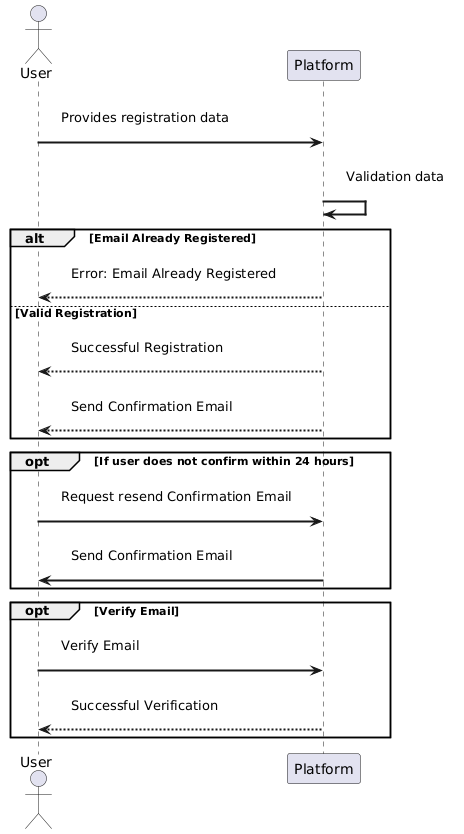
\includegraphics[scale = 0.8]{Images/ImagesRASD/user_registration.png}
\end{center}
\newpage
\textbf{2) User Login}\\

\begin{table}[h!]
    \centering
    \begin{tabular}{lp{10cm}}
        \textbf{Actor} & User \\ \hline
        \textbf{Entry conditions} & The user is on the login page of the S\&C platform, ready to enter credentials. \\ \hline
        \textbf{Event Flow} & 
        1. The user enters their email and password. \\
        & 2. The S\&C platform validates the credentials. \\
        & 3a. If the credentials are valid, the platform successfully logs in the user. \\
        & 3b. If the credentials are invalid, the platform returns an error: "Invalid email or password, please try again." \\
        \hline
        \textbf{Exit condition} & The user is logged into the platform if the credentials are valid. \\ \hline
        \textbf{Exceptions} & 
        3.1. Invalid email or password: the user must re-enter the correct credentials to log in. \\
    \end{tabular}
    \caption{User login use case}
    \label{tab:user_login}
\end{table}


\begin{center}
    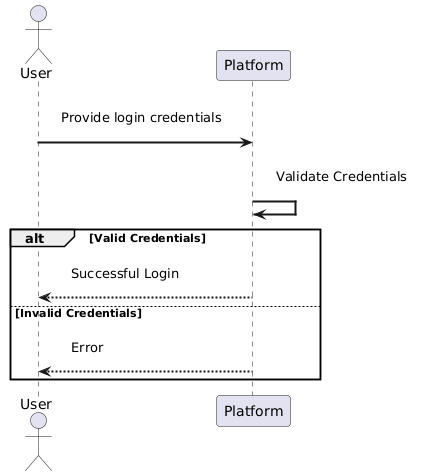
\includegraphics[scale = 1]{Images/ImagesRASD/user_login.png}
\end{center}

\newpage
\textbf{3) Internship post creation use case}\\

\begin{table}[h!]
    \centering
    \begin{tabular}{lp{10cm}}
        \textbf{Actor} & Company \\ \hline
        \textbf{Entry conditions} & The company is on the S\&C platform, ready to create a new internship post. \\ \hline
        \textbf{Event Flow} & 
        1. The company fills out the internship information form. \\
        & 2. The S\&C platform validates the internship data. \\
        & 3a. If the data is valid, the platform creates the new internship post and confirms success to the company. \\
        & 3b. If the data is invalid, the platform returns an error: "Error in internship data, please correct the form." \\
        & 4. The company resubmits the corrected form, repeating the process until valid data is provided. \\
        & 5. The platform performs matching to find relevant students for the internship post. \\
        & 6. For each student that matches, the platform sends an internship post notification. \\
        \hline
        \textbf{Exit condition} & A new internship post is successfully created on the platform, and notifications are sent to relevant students. \\ \hline
        \textbf{Exceptions} & 
        3.1. Invalid internship data: The company must correct and resubmit the form until valid data is provided. \\
    \end{tabular}
    \caption{Internship post creation use case}
    \label{tab:internship_post_creation}
\end{table}



\begin{center}
    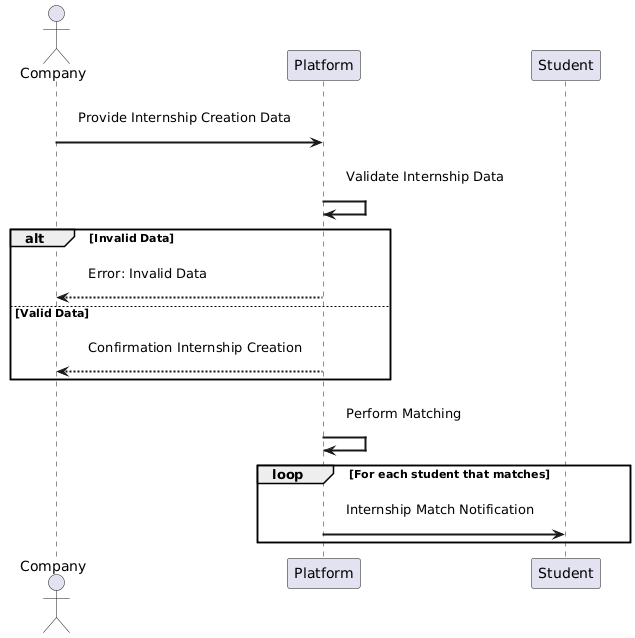
\includegraphics[scale = 0.8]{Images/ImagesRASD/Internship_post_creation_use_case.png}
\end{center}

\newpage
\textbf{4) Personal data and CV upload use case}\\

\begin{table}[h!]
    \centering
    \begin{tabular}{lp{10cm}}
        \textbf{Actor} & Student \\ \hline
        \textbf{Entry conditions} & The student is on the S\&C platform, ready to submit personal data and optionally upload a CV. \\ \hline
        \textbf{Event Flow} & 
        1. The student submits their skills, interests, and other personal data. \\
        & 2a. If the personal data is invalid, the platform returns an error: "Error in personal data, please correct it." \\
        & 2b. If the personal data is valid, the platform confirms that the data was successfully uploaded. \\
        & 3. The student optionally uploads their CV. \\
        & 4a. If the CV is invalid, the platform returns an error: "Error in CV, please re-upload." \\
        & 4b. If the CV is valid, the platform confirms that the upload was successful. \\
        & 5. The platform performs matching based on the student data. \\
        & 6. For each matching company, the platform sends a notification about the student. \\
        \hline
        \textbf{Exit condition} & The student's personal data and, if applicable, CV are successfully uploaded and relevant companies are notified. \\ \hline
        \textbf{Exceptions} & 
        2.1. Invalid personal data: The student must correct and resubmit their personal data. \\
        & 4.1. Invalid CV: The student must re-upload their CV until it meets the platform's requirements. \\
    \end{tabular}
    \caption{Student personal data and CV upload use case}
    \label{tab:student_data_cv_upload}
\end{table}



\begin{center}
    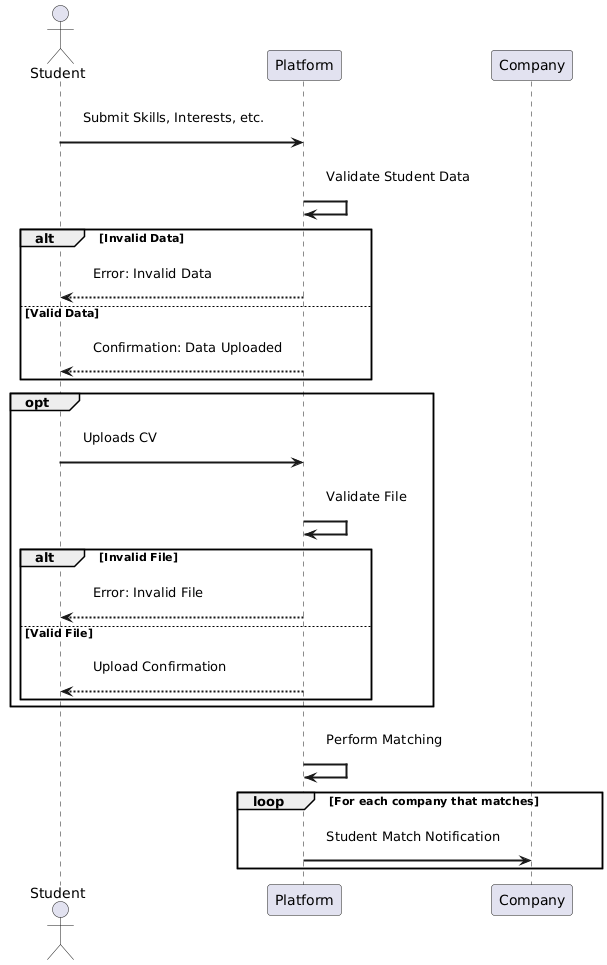
\includegraphics[scale = 0.7]{Images/ImagesRASD/Personal_data_and_CV_upload.png}
\end{center}

\newpage
\textbf{5) Student application use case}\\

\begin{table}[h!]
    \centering
    \begin{tabular}{lp{10cm}}
        \textbf{Actor} & Student \\ \hline
        \textbf{Entry conditions} & The student is on the S\&C platform, ready to apply for an internship. \\ \hline
        \textbf{Event Flow} & 
        1. The student requests a list of internships. \\
        & 2. The platform provides the list of available internships. \\
        & 3. The student selects an internship from the list. \\
        & 4. The platform displays the details of the selected internship. \\
        & 5. The student submits their application data for the selected internship. \\
        & 6. The platform validates the application data. \\
        & 7a. If the data is valid, the platform confirms that the application submission was successful. \\
        & 7b. If the data is not valid, the platform returns an error message. \\
        & 8. If valid, the platform sends the application to the company. \\
        \hline
        \textbf{Exit condition} & The student's application for the internship is successfully submitted and sent to the company if the data is valid. \\ \hline
        \textbf{Exceptions} & 
        7.1. Invalid application data: The student must correct and resubmit their application data until it meets the platform's requirements. \\
    \end{tabular}
    \caption{Internship application use case}
    \label{tab:internship_application}
\end{table}


\begin{center}
    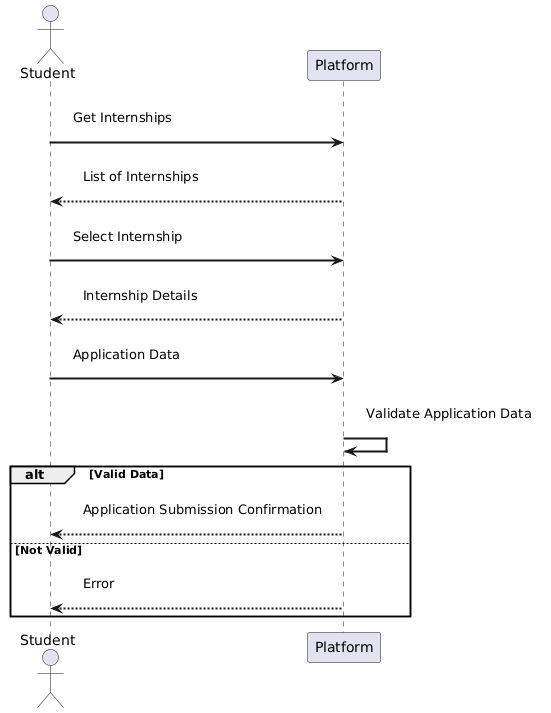
\includegraphics[scale = 0.8]{Images/ImagesRASD/Student_application.png}
\end{center}

\newpage
\textbf{6) Company to manage income applications}\\

\begin{table}[h!]
    \centering
    \begin{tabular}{lp{10cm}}
        \textbf{Actor} & Company \\ \hline
        \textbf{Entry conditions} & The company is on the S\&C platform, ready to manage internship applications. \\ \hline
        \textbf{Event Flow} & 
        1. The company requests the list of internship posts. \\
        & 2. The platform provides the list of posted internships. \\
        & 3. The company selects a specific internship from the list. \\
        & 4. The platform displays the details of the selected internship. \\
        & 5. The company requests the list of applicants for the internship. \\
        & 6. The platform provides the list of applicants. \\
        & 7. For each application: \\
        & \quad a. The company requests applicant information. \\
        & \quad b. The platform provides the applicant information. \\
        & \quad c. The company reviews the selected application. \\
        & \quad d. The platform displays the status result. \\
        & \quad e. The company updates the status on the platform. \\
        & \quad f. The platform sends the result to the student. \\
        \hline
        \textbf{Exit condition} & The company's review and status update for each applicant are completed, and results are sent to students. \\ \hline
        \textbf{Exceptions} & None specified. \\
    \end{tabular}
    \caption{Company management of internship applications use case}
    \label{tab:company_manage_internship_applications}
\end{table}


\begin{center}
    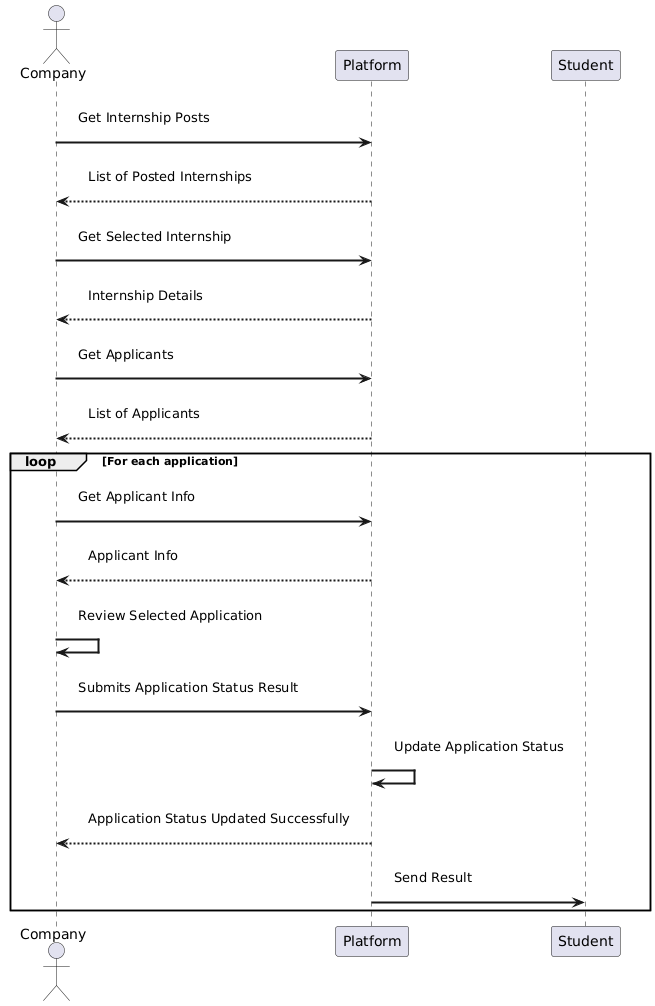
\includegraphics[scale = 0.7]{Images/ImagesRASD/Company_to_manage_income_applications.png}
\end{center}

\newpage
\textbf{7) Student sending answer use case}\\

\begin{table}[h!]
    \centering
    \begin{tabular}{lp{10cm}}
        \textbf{Actor} & Student \\ \hline
        \textbf{Entry conditions} & The student is on the platform and ready to respond to questions. \\ \hline
        \textbf{Event Flow} & 
        1. The student responds to each question individually. \\
        & 2. After answering all questions, the student sends their answers to the platform. \\
        & 3. The platform validates the submitted answers. \\
        & 4a. If the answers are valid, the platform saves the answers and sends a confirmation to the student. \\
        & 4b. If the answers are not valid, the platform sends an error message to the student indicating that revision is needed. \\
        \hline
        \textbf{Exit condition} & The student's answers are successfully validated and saved on the platform, or the student is notified to revise the answers. \\ \hline
        \textbf{Exceptions} & 
        4.1. Invalid answers: The student must revise and resubmit their answers until they meet the platform's requirements. \\
    \end{tabular}
    \caption{Student answer submission and validation use case}
    \label{tab:student_answer_submission}
\end{table}


\begin{center}
    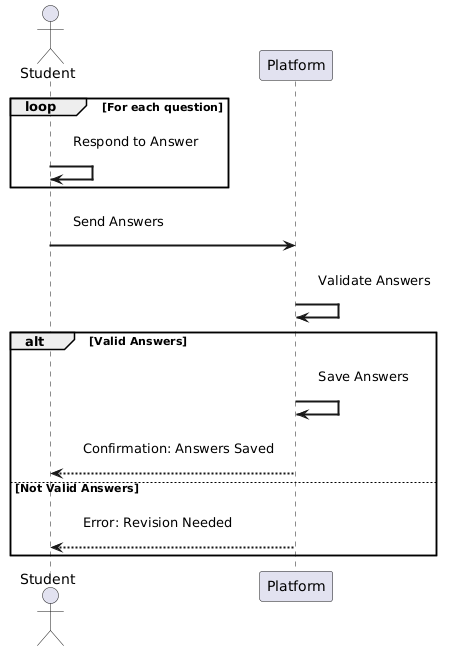
\includegraphics[scale = 0.8]{Images/ImagesRASD/Student_sending_answers.png}
\end{center}

\newpage
\textbf{8) Company questions reviewing}\\

\begin{table}[h!]
    \centering
    \begin{tabular}{lp{10cm}}
        \textbf{Actor} & Company \\ \hline
        \textbf{Entry conditions} & The company is on the platform and ready to manage internship applications. \\ \hline
        \textbf{Event Flow} & 
        1. The company requests the list of internship posts. \\
        & 2. The platform provides the list of posted internships. \\
        & 3. The company selects a specific internship from the list. \\
        & 4. The platform displays the details of the selected internship. \\
        & 5. The company requests the list of applicants for the internship. \\
        & 6. The platform provides the list of applicants. \\
        & 7. For each applicant: \\
        & \quad a. The company requests the applicant's answers. \\
        & \quad b. The platform provides the applicant's answers. \\
        & \quad c. The company reviews the applicant's answers. \\
        & \quad d. The company stores the result on the platform. \\
        & \quad e. The platform displays the result to the company. \\
        & \quad f. The company updates the status and notifies the applicant. \\
        & \quad g. The platform sends the result to the student. \\
        \hline
        \textbf{Exit condition} & The company's review and status update for each applicant are completed, and results are sent to the students. \\ \hline
        \textbf{Exceptions} & None specified. \\
    \end{tabular}
    \caption{Company management of internship applications use case}
    \label{tab:company_manage_internship_applications}
\end{table}

\begin{center}
    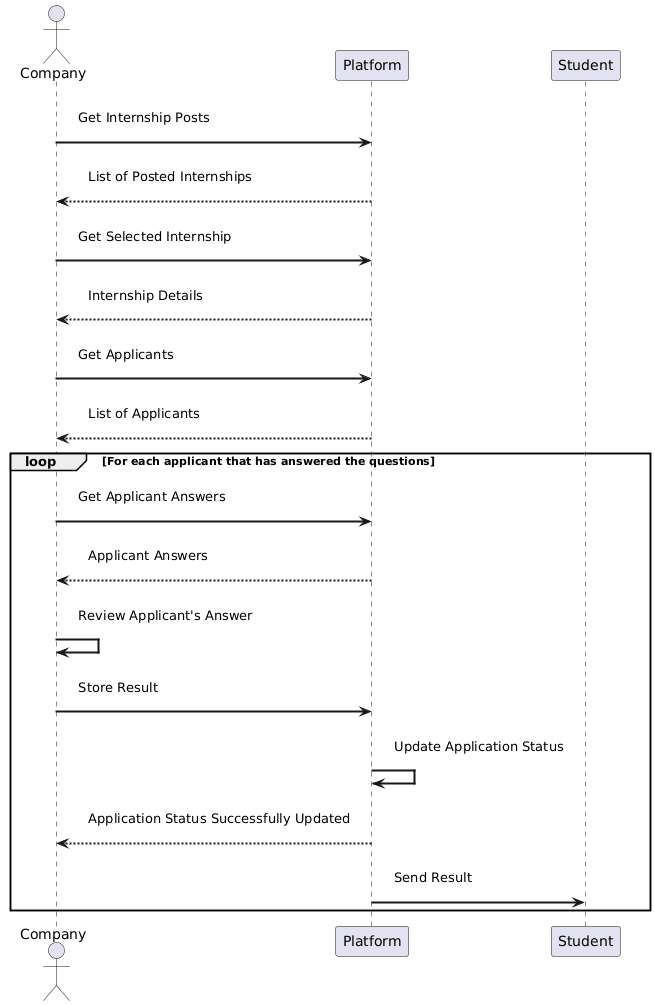
\includegraphics[scale = 0.8]{Images/ImagesRASD/Company_questions_reviewing.png}
\end{center}

\newpage
\subsection{Summary of the Functional Requirements}
\begin{longtable}{|p{0.1\textwidth}|p{0.9\textwidth}|}
\hline
\textbf{R1} & The S\&C shall allow students to view a personalized dashboard displaying recommended internships, application statuses, and feedback. \\ 
\hline
\textbf{R2} & The S\&C shall allow students to create and edit profiles, upload CVs, and receive real-time validation. \\ 
\hline
\textbf{R3} & The S\&C shall allow students to access a search tool with filtering options for location, field of study, and required skills. \\ 
\hline
\textbf{R4} & The S\&C shall allow students to be guided through the application process with a step-by-step wizard, displaying deadlines and tracking progress. \\ 
\hline
\textbf{R5} & The S\&C shall allow companies to create, edit, and delete internship postings, including job roles and required skills. \\ 
\hline
\textbf{R6} & The S\&C shall allow companies to have a dashboard to review candidate applications, filter profiles, and schedule interviews. \\ 
\hline
\textbf{R7} & The S\&C shall allow companies to have a recommendation feed for candidates based on internship requirements. \\ 
\hline
\textbf{R8} & The S\&C shall allow universities to have an administrative dashboard to monitor internship progress and manage complaints. \\ 
\hline
\textbf{R9} & The S\&C shall allow universities to log, track, and update complaint statuses within a complaint management system. \\ 
\hline
\textbf{R10} & The S\&C shall allow integration with university databases via secure Restful APIs for verifying student enrollment and monitoring internship progress. \\ 
\hline
\textbf{R11} & The S\&C shall allow API integration with external career platforms and feedback tools for gathering insights on internship performance. \\ 
\hline
\textbf{R12} & The S\&C shall allow push notifications for web and mobile platforms, notifying users in real-time. \\ 
\hline
\textbf{R13} & The S\&C shall allow students to create and manage profiles, including personal details, education history, skills, and work experience. \\ 
\hline
\textbf{R14} & The S\&C shall allow companies to specify deadlines for internship postings, with automatic removal of expired listings. \\ 
\hline
\textbf{R15} & The S\&C shall allow the recommendation engine to improve over time based on feedback from student internships. \\ 
\hline
\textbf{R16} & The S\&C shall allow companies to manage interview schedules and log outcomes, including scores and feedback. \\ 
\hline
\textbf{R17} & The S\&C shall allow both students and companies to provide feedback post-internship, covering skills demonstrated and overall satisfaction. \\ 
\hline
\textbf{R18} & The S\&C shall allow universities to access a complaint management system for reviewing and resolving student-company issues. \\ 
\hline
\textbf{R19} & The S\&C shall allow a secure messaging system for direct communication between students and companies while preserving user privacy. \\ 
\hline
\textbf{R20} & The S\&C shall allow companies access to a comprehensive analytics dashboard to analyze candidate engagement, track application trends, and optimize postings. \\ 
\hline
\textbf{R21} & The S\&C shall allow students to set career goals and objectives, with tailored internship suggestions based on these goals. \\ 
\hline
\textbf{R22} & The S\&C shall allow users to select their preferred language from platform settings to enhance accessibility. \\ 
\hline
\textbf{R23} & The S\&C shall allow companies to access a "Similar Candidates" feature to view potential matches based on applicant profiles. \\ 
\hline
\textbf{R24} & The S\&C shall allow a feedback mechanism for students to receive suggestions for improving profiles, including skill recommendations based on industry trends. \\ 
\hline
\textbf{R25} & The S\&C shall allow students and companies to rate each other post-internship, contributing to a reputation score visible to other users. \\ 
\hline
\textbf{R26} & The S\&C shall allow a periodic internship recommendation email digest for students who opt-in, summarizing new or high-match opportunities. \\ 
\hline
\textbf{R27} & The S\&C shall allow students to track essential pre- and post-internship tasks and documents with a "Checklist" tool. \\ 
\hline
\textbf{R28} & The S\&C shall allow companies access to templates and guidelines for internship descriptions to standardize postings and engage suitable candidates. \\ 
\hline
\textbf{R29} & The S\&C shall allow students to recommend other students for internships, fostering peer networking through a referral feature. \\ 
\hline
\textbf{R30} & The S\&C shall allow integration of two-factor authentication for enhanced security of student and company accounts. \\ 
\hline
\textbf{R31} & The S\&C shall allow encryption of all sensitive user data, ensuring compliance with data protection regulations. \\ 
\hline
\textbf{R32} & The S\&C shall allow a help center with FAQs and live chat support for real-time assistance for students, companies, and university administrators. \\ 
\hline
\textbf{R33} & The S\&C shall allow automated reminders for companies about pending feedback or assessments for completed internships. \\ 
\hline
\textbf{R34} & The S\&C shall allow students to mark internships as "favorites" or for easy reference during application. \\ 
\hline
\textbf{R35} & The S\&C shall allow companies to post exclusive internships targeted to students from specific universities or programs. \\ 
\hline
\textbf{R36} & The S\&C shall allow students access to an analytics page showing internship trends, including popular industries, roles, and demanded skills. \\ 
\hline
\textbf{R37} & The S\&C shall allow students and companies access to a document management tool for secure uploading, storing, and sharing of internship-related documents. \\ 
\hline
\textbf{R38} & The S\&C shall allow companies to set internship visibility criteria, such as grade level, skill sets, and field of study. \\ 
\hline
\textbf{R39} & The S\&C shall allow universities access to an analytics dashboard to track student engagement, successful matches, and completion rates. \\ 
\hline
\textbf{R40} & The S\&C shall allow a reporting feature for users to report inappropriate or irrelevant internship environment, ensuring a safe and professional place. \\ 
\hline
\textbf{R41} & The S\&C shall allow personalized reminders for students, notifying them of application deadlines, interview dates, and required documents. \\ 
\hline
\textbf{R42} & The S\&C shall allow students to set privacy levels on their profiles, determining what details are public to companies or universities. \\  
\hline
\textbf{R43} & The S\&C shall allow integration with calendars for synchronizing dates like interview or deadline dates. \\ 
\hline
\textbf{R44} & The S\&C shall allow a section with the best internship sorted by feedbacks. \\ 
\hline
\textbf{R45} & The S\&C shall allow students to view average application review times by companies via an "Application Insights" feature. \\ 
\hline
\textbf{R46} & The S\&C shall allow an assessment tool for students to understand and showcase non-technical strengths. \\ 
\hline
\textbf{R47} & The S\&C shall allow tracking of job market trends, notifying students of growing fields to help adapt skills according to their matching features. \\ 
\hline
\textbf{R48} & The S\&C shall allow endorsements from companies and universities, adding credibility to student profiles for specific skills. \\ 
\hline
\textbf{R49} & The S\&C shall allow a real-time "Internship Analytics" page for universities, summarizing internship data like completion rates. \\ 
\hline
\textbf{R50} & The S\&C shall allow companies a Candidate Comparison tool for side-by-side candidate evaluation. \\ 
\hline
\textbf{R51} & The S\&C shall allow real-time tracking of application statuses, showing students the progress of applications at each stage. \\ 
\hline
\textbf{R52} & The S\&C shall allow a recommendation ranking feature to help students prioritize opportunities based on match percentage and goals. \\ 
\hline
\textbf{R53} & The S\&C shall allow an internship recommendation score based on student profiles, skills. \\ 
\hline
\textbf{R54} & The S\&C shall allow companies to provide additional criteria\\
\hline
\end{longtable}
\newpage
\subsection{Mapping on Goals}
In the following table it is shown how the different goals map on the requirements and domain assumptions described in the previous chapters. Furthermore, the mapping is made in order to make this formula hold 
\begin{equation}
R \land D \models G
\end{equation}
\begin{longtable}{| p{0.3\textwidth} | p{0.4\textwidth} | p{0.3\textwidth} |}
\hline
\textbf{Goal} & \textbf{Domain Assumptions (DA)} & \textbf{Requirements (R)} \\ 
\hline
G1: Enable students to search for internships that match their skills and career goals. & DA1: Students need internships to gain practical experience. \newline DA3: Students have varied skills and interests. \newline DA5: Students need to provide a valid email address. \newline DA8: Both students and companies need to have a connection and a device to connect to the platform. & R1: Display a personalized dashboard with recommended internships, application statuses, and feedback. \newline R2: Allow students to create/edit profiles, upload CVs, and validate them in real-time. \newline R3: Provide a search tool with filtering options. \newline R4: Guide students through applications with a step-by-step wizard. \newline R21: Enable students to set career goals and receive tailored internship suggestions. \newline R52: Provide a recommendation ranking feature to help students prioritize opportunities. \\ \hline

G2: Provide companies with tools to advertise internships and attract suitable candidates. & DA2: Companies need interns for various projects. \newline DA4: Companies have specific internship requirements. \newline DA6: Companies need to provide a valid email. \newline DA8: Both parties need connectivity to the platform. & R5: Enable companies to manage internship postings with job roles and skill requirements. \newline R6: Provide a dashboard for companies to review applications, filter profiles, and schedule interviews. \newline R14: Allow companies to specify deadlines for postings, with expired listings automatically removed. \newline R20: Give companies access to analytics for candidate engagement and application trends. \newline R28: Provide templates and guidelines to standardize internship descriptions. \newline R38: Allow companies to set visibility criteria based on grade level, skills, and field of study. \\ \hline

G3: Offer recommendation mechanisms for students to match with relevant internships. & DA3: Students have varied skills and interests. \newline DA4: Companies have specific internship requirements. & R7: Provide companies with a recommendation feed based on internship requirements. \newline R15: Improve the recommendation engine over time based on feedback from completed internships. \newline R21: Allow students to set career goals for more tailored suggestions. \newline R52: Enable students to prioritize opportunities with a ranking feature. \newline R53: Generate internship recommendation scores based on student profiles and past performance. \\ \hline

G4: Offer recommendation mechanisms for companies to find potential candidates. & DA2: Companies need interns for various projects. \newline DA4: Companies have specific internship requirements. & R6: Provide companies with a dashboard to review applications and filter profiles. \newline R7: Offer companies a recommendation feed for candidates. \newline R23: Show companies "Similar Candidates" based on profiles. \newline R50: Include a "Candidate Comparison" tool for companies to evaluate applicants side-by-side. \\ \hline

G5: Facilitate the selection process through an interview management system. & DA2: Companies need interns for various projects. \newline DA4: Companies have specific internship requirements. & R5: Enable companies to create and manage internship postings. \newline R6: Provide companies a dashboard to review and manage candidate applications. \newline R16: Support interview scheduling and logging, including scores and feedback. \newline R20: Include a comprehensive analytics dashboard for tracking trends. \newline R68: Allow additional selection criteria like language requirements. \\ \hline

G6: Supports the candidate's evaluation. & DA4: Companies have specific internship requirements. \newline DA9: Universities are interested in monitoring internship quality. & R16: Support interview scheduling and recording outcomes. \newline R17: Enable feedback mechanisms post-internship for skills and satisfaction. \newline R50: Provide a comparison tool for side-by-side candidate evaluation. \\ \hline

G7: Gather feedback from students and companies to continuously improve the matchmaking process. & DA3: Students have varied skills and interests. \newline DA4: Companies have specific internship requirements. \newline DA9: Universities are interested in monitoring internship quality. & R15: Continuously improve the recommendation engine with feedback. \newline R17: Facilitate feedback post-internship. \newline R24: Offer profile improvement suggestions, including skill recommendations. \newline R33: Send automated reminders for companies to provide feedback. \newline R44: Include a "Success Stories" section showcasing successful internships. \\ \hline

G8: Enable universities to monitor internship progress and manage potential issues. & DA9: Universities are interested in monitoring internship quality. \newline DA7: Universities need to have a valid email. & R8: Allow universities to access an administrative dashboard for monitoring. \newline R9: Provide a complaint management system for universities. \newline R10: Integrate with university databases for student verification and internship progress monitoring. \newline R39: Enable universities to access analytics on engagement and completion rates. \newline R49: Show universities a real-time "Internship Analytics" page summarizing internship data. \\ \hline
\end{longtable}



\begin{itemize}
    \item \textbf{Student Profile Management}: 
        \begin{itemize}
            \item Students can create and manage profiles, including personal details, education history, skills, and work experience.
            \item The profile interface will support dynamic updates, and validation of critical fields to ensure profile completeness.
            \item Uploaded CVs must be in PDF or DOCX format, and the system must validate that the upload meets the required format.
            \item Profiles must support a review system where students can preview how their information will appear to potential employers.
        \end{itemize}
    \item \textbf{Internship Listings}: 
        \begin{itemize}
            \item Companies can create, update, and delete internship listings with detailed descriptions, requirements, and benefits.
            \item Listings must include filters for location, skills, and compensation, allowing students to search effectively.
            \item The system must allow companies to specify internship deadlines, and automatically remove expired listings.
            \item A dynamic feedback mechanism will notify companies about the completeness and attractiveness of their internship postings, suggesting improvements if needed.
        \end{itemize}
    \item \textbf{Recommendation System}: 
        \begin{itemize}
            \item The recommendation engine must take into account factors such as the student’s skills, location preferences, previous internships, and company requirements.
            \item The engine will learn and improve over time using feedback data from previous internships, adjusting future recommendations based on the outcomes and feedback provided by both students and companies.
        \end{itemize}
    \item \textbf{Selection and Interview Process}: 
        \begin{itemize}
            \item Companies can select candidates for interviews and manage interview schedules directly through the platform.
            \item Structured questionnaires will be provided by companies for student applicants to complete prior to interviews, with results stored in the system for company review.
            \item Companies will be able to log interview outcomes, including scores and qualitative feedback, directly into the system to aid decision-making.
        \end{itemize}
    \item \textbf{Feedback Collection}: 
        \begin{itemize}
            \item After each internship, both students and companies must provide structured feedback on the experience.
            \item The feedback must cover multiple dimensions, including skills demonstrated, professionalism, and overall satisfaction.
            \item The system will anonymize feedback to comply with GDPR regulations, ensuring privacy for both parties involved.
            \item The feedback will be used as a data source for improving the recommendation system and internship matching algorithm.
        \end{itemize}
    \item \textbf{Complaint Handling}: 
        \begin{itemize}
            \item Universities must have access to a complaint management system, allowing them to view and manage complaints filed by either students or companies.
            \item Complaints must be classified by type (e.g., harassment, contract breach) and tracked through a resolution workflow.
            \item Complaints can be escalated for review by a university administrator, who will have access to the full history of the issue.
            \item The system will automatically notify all relevant parties (students, companies, administrators) of complaint status updates.
        \end{itemize}
\end{itemize}

\section{Performance Requirements}

\subsection{Number of Users}
The platform will be used by multiple parties, including students, companies, and universities. Based on market research, which includes a comparison with existing similar platforms such as the CareerService platform for Politecnico di Milano (Polimi) and other internship-matching services across Europe, we estimate that S\&C will attract approximately 20,000 students and 2,500 companies from various universities and industries. Additionally, around 50 universities will be actively using the platform to monitor internships. This gives us an estimated total user base of 22,550 users.\\ \\
Considering a worst-case scenario where 40\% of the users are active simultaneously, the system must support up to 9,020 concurrent users. The platform must ensure smooth operation, even during peak usage times.

\subsection{Data Storage}
The platform needs to store various types of data related to students, companies, internships, and the matchmaking process. Below are the estimated storage requirements for the first year of operation:

\begin{itemize}
    \item \textbf{Student data (profile)}: Each student will have a profile containing personal information such as name, contact details, and skillset. This profile data is estimated to require around 10 KB per student. Considering 20,000 students:
    \[
    20,000 \times 10 \, \text{KB} = 195.3 \, \text{MB}
    \]
    
    \item \textbf{Student data (PDF CVs)}: In addition to the basic profile information, each student is expected to upload their CV in PDF format. The average size of a CV in PDF format is estimated to be around 300 KB. Thus, for 20,000 students:
    \[
    20,000 \times 300 \, \text{KB} = 5.72 \, \text{GB}
    \]
    
    \item \textbf{Company data}: Each company will have a profile including company information, project descriptions, and internship offerings. Assuming 15 KB of storage per company profile and considering 2,500 companies:
    \[
    2,500 \times 15 \, \text{KB} = 36.6 \, \text{MB}
    \]
    
    \item \textbf{Internship postings}: Each internship posting will include information about the project, tasks, technologies, and terms (e.g., paid/unpaid). Assuming each posting requires 10 KB and that each company posts five internships a year:
    \[
    2,500 \times 5 \times 10 \, \text{KB} = 122.1 \, \text{MB}
    \]
    
    \item \textbf{Student feedback and internship outcomes}: Feedback data provided by students and companies will be stored for analysis. Assuming 5 KB per feedback submission and expecting each internship to receive three feedback entries, for 10,000 matched internships in the first year:
    \[
    10,000 \times 3 \times 5 \, \text{KB} = 146.5 \, \text{MB}
    \]
    
    \item \textbf{Interview and selection data}: Information about interviews, questionnaires, and selection processes will also be stored. Assuming 8 KB per interview record and that each company interviews an average of five candidates per internship:
    \[
    10,000 \times 5 \times 8 \, \text{KB} = 390.6 \, \text{MB}
    \]
\end{itemize}

Summing all storage requirements for the first year:
\[
195.3 \, \text{MB} + 5.72 \, \text{GB} + 36.6 \, \text{MB} + 122.1 \, \text{MB} + 146.5 \, \text{MB} + 390.6 \, \text{MB} = 6.6 \, \text{GB}
\]\\
Thus, a storage allocation of \textbf{10 GB} will be sufficient to accommodate the platform's data storage needs for a year, including room for growth and additional data generated by the system.


\subsection{Time Response}
Although there are no strict time requirements for the S\&C platform, it is important to maintain a responsive user experience. Reasonable average response times for key interactions could be as follows:
\begin{itemize}
    \item Basic search queries and browsing operations should ideally be processed within \textbf{2 seconds}, to ensure a smooth navigation experience.
    \item More complex operations, such as generating personalized internship recommendations, should aim to complete within \textbf{5 seconds}, balancing the computational effort required with acceptable wait times for the user.
\end{itemize}

\section{Design Constraints}

\subsection{Standards Compliance}

The platform must adhere to EU's GDPR regulations to ensure secure data storage and transmission, particularly when handling sensitive student and company data. All data interactions must comply with GDPR provisions regarding data ownership, user consent, and the right to access and delete data.

Additionally, the platform must comply with industry security standards to ensure the system is secure against potential threats.

\subsection{Hardware Limitations}

There are no specific hardware limitations imposed on end-users.

\section{Software System Attributes}

\subsection{Reliability}
The S\&C platform must be reliable to ensure continuous operation, even in the presence of faults. The system should be designed to be fault-tolerant to prevent the propagation of errors and ensure uninterrupted usability. Mechanisms such as automated failover and data redundancy should be in place to mitigate the risk of downtime due to unexpected failures.

\subsection{Availability}
The platform must be available as much as possible, with a minimum uptime of 99.999\%. Scheduled maintenance breaks should be minimized and, when necessary, performed during low-traffic periods (e.g., nighttime) to avoid disrupting critical usage, particularly around high-demand periods such as internship application deadlines.

\subsection{Security}
Security is critical for the S\&C platform, as it handles sensitive student and company data. The system must implement strong authentication and authorization mechanisms. Authentication should ensure that users are properly identified before accessing the platform, while authorization should ensure that users can only perform actions they are permitted to.

\subsection{Maintainability}
The platform should be designed with scalability and modularity in mind to facilitate the easy addition of new features or modifications with minimal effort. The use of reusable code components and modular architecture will aid in making future updates efficient. Regular maintenance operations should be scheduled during times of low user activity, such as nighttime, to minimize disruptions to users.

\subsection{Portability}
The S\&C platform must be accessible from a wide range of web browsers, ensuring compatibility across all major platforms (e.g., Chrome, Firefox, Safari, and Edge). On the client side, the platform should support responsive design, making it accessible on both desktop and mobile devices. No specific portability requirements are imposed on the server side, provided the platform can run on common server configurations.


\newpage


\chapter{Formal Analysis}
\begin{lstlisting}
//ENUMERATIONS +++++++++++++++++++++++++++++++++++++++++++++++++++

enum ApplicationStatus { LastEvaluation, Rejected, Screening, OnlineAssessment, Accepted }
enum QuestionType { MultipleChoice, OpenQuestion, TrueOrFalse }
enum InternshipDuration { TwoToThreeMonths, ThreeToSixMonths, SixToTwelveMonths, MoreThanOneYear }
enum AnswerStatus {Completed, Uncompleted}

//SIGNATURE +++++++++++++++++++++++++++++++++++++++++++++++++++


abstract sig User{
    email: disj one Email,
    password: disj one Password
}

sig Student extends User{
	cv: disj one CV,
	appliedTo: Internship,
	skills: some Skills,
	feedback_of_internship: Internship -> some Feedback,
	feedback_of_platform: Feedback,
	enrolled: one University
 }

sig University extends User{
	tracked_internship : Student -> Internship,
	tracked_feedback : Internship -> Feedback,
	feedback_of_internship : Feedback -> Internship
}{this in Student.enrolled}


sig Company extends User {
    	feedback_of_internship: Feedback -> Internship,
	feedback_of_platform: Feedback
}

sig Internship{
	suitable_skills: set Skills,
	feedback_internship: disj set Feedback,
	questions: set Internship_Question,
	applications: disj set Student -> Application
}

sig Application{
	title: String,
	description: String,
	status: ApplicationStatus,
	forInternship: one Internship,
	answers: set Answer
}

sig Internship_Question{
	has_questions: set Question,
}{this in Internship.questions}

sig Match{
	match: Student -> some Internship
}

sig Skills{}


sig Question {
	answer: disj one Answer,
	type: QuestionType
}{this in Internship_Question.has_questions}

sig Answer {
	completed: one Bool
}

sig Feedback {}

sig Email {}
sig Password {}

sig CV {
}{this in Student.cv}


enum Bool {True, False}

//FACT
//++++++++++++++++++++++++++++++++++++++++++//

fact ApplicationMustHaveStatus{
	all a: Application |
		one a.status
}


//Match between student and internship needs to have the same preferences
fact SameMatchSamePreferences{
	all m: Match | all s: Student | all i: Internship |
		s->i in m.match iff #(s.skills & i.suitable_skills) != 0
}



//Intersection between match and application must be empty
fact MatchAndApplicationDisjoint {
    all s: Student, i: Internship|
        (s -> i in Match.match) implies not (i in (s.appliedTo))
}


//A student cannot apply to the same application more than one time
fact MaximumOneApplicationPerIntership{
	all s : Student
| no i : Internship | i in (s.appliedTo) and #(i & (s.appliedTo)) > 1
}


//Internship question must be a subset of question
fact InternshipQuestionsSubset {
    all iq: Internship_Question | iq.has_questions in Question
}

//In order to have an Accepted_Application all answer must be completed
fact AllAnswersMustBeCompletedForAcceptedApplication {
	all i: Internship| all q: Question| all s: Student |
	s.((i.applications).status) in Accepted implies q in i.questions.has_questions and q.answer.completed in True
}

//The answer are available only in an Accepted_Application status
fact AnswersOnlyInAcceptedApplication {
    all i: Internship, s: Student | 
        some i.questions.has_questions implies s.((i.applications).status) in Accepted
}


//Application has feedback only if its status is either Accepted_Application or Rejected_Application
fact FeedbackOnlyForAcceptedOrRejectedApplication {
    all s: Student | all i: Internship |
        some i.(s.feedback_of_internship) implies s.((i.applications).status) in Accepted or s.((i.applications).status) in Rejected
}


//Cannot add feedback to application which are not Accepted_Application
fact NoFeedbackForNonAcceptedApplication {
    all i: Internship, s: Student |
        some i.feedback_internship implies (s.(i.applications).status) in Accepted
}

//PREDICATES
//+++++++++++++++++++++++++++++++++++++++++++++++++++++++++++++++++++

//User add a CV
pred StudentAddCV[s: Student, cv_new: CV]
{
	s.cv = s.cv + cv_new
} 

//User remove a CV
pred StudentRemoveCV[s: Student, cv_to_remove: CV]
{
	s.cv = s.cv - cv_to_remove
}

//New Match has been found between a student and internship and added
pred AddNewMatch(s: Student, i: Internship, m: Match) {
    s -> i in m.match
    and s.skills & i.suitable_skills != none
}

//New feedback for an internship has been added by a student
pred NewFeedbackStudent[f_new: Feedback, s: Student, i: Internship]
{
    i.(s.feedback_of_internship) = i.(s.feedback_of_internship) + f_new
}

//New feedback has been added by a company
pred NewFeedbackCompany[f_new: Feedback, c: Company, i: Internship]
{
    (c.feedback_of_internship).i = (c.feedback_of_internship).i + f_new
}

//Every student's feeback must be tracked by his university
fact UniversityTracksFeedback {
    all s: Student, i: Internship, u: University |
        some i.(s.feedback_of_internship) implies i.(u.tracked_feedback) = i.(s.feedback_of_internship)
}

// Ensure the university tracks internships for students who have provided feedback
fact UniversityTracksInternships {
    all s: Student, i: Internship, u: University |
        some i.(s.feedback_of_internship) implies i in s.(u.tracked_internship)
}



//ASSERTION +++++++++++++++++++++++++++++++++++++++++++++++++++

assert FeedbackConsistency {
    all i: Internship | all s: Student |  all u: University |
    (i in (s.appliedTo) and #(i.(s.feedback_of_internship)) != 0) implies 
     i.(u.tracked_feedback) = i.(s.feedback_of_internship) and i in s.(u.tracked_internship)
}

assert ValidMatch {
    all m: Match | all s: Student | all i: Internship |
    s -> i in m.match implies s.skills & i.suitable_skills != none
}


pred simpleWorld{
	#Student = 1
	#University = 1
	#Company = 1
	#Internship = 2
	#Internship_Question = 1
	#Question = 1
	#Skills = 1
}

//TO RUN ASSERTION AND PREDICATES

run StudentAddCV for 4

run StudentRemoveCV for 4

run AddNewMatch for 4

run NewFeedbackStudent for 4

run NewFeedbackCompany for 4

check FeedbackConsistency

check ValidMatch

run simpleWorld for 5


\end{lstlisting}



\begin{figure}
    \centering
    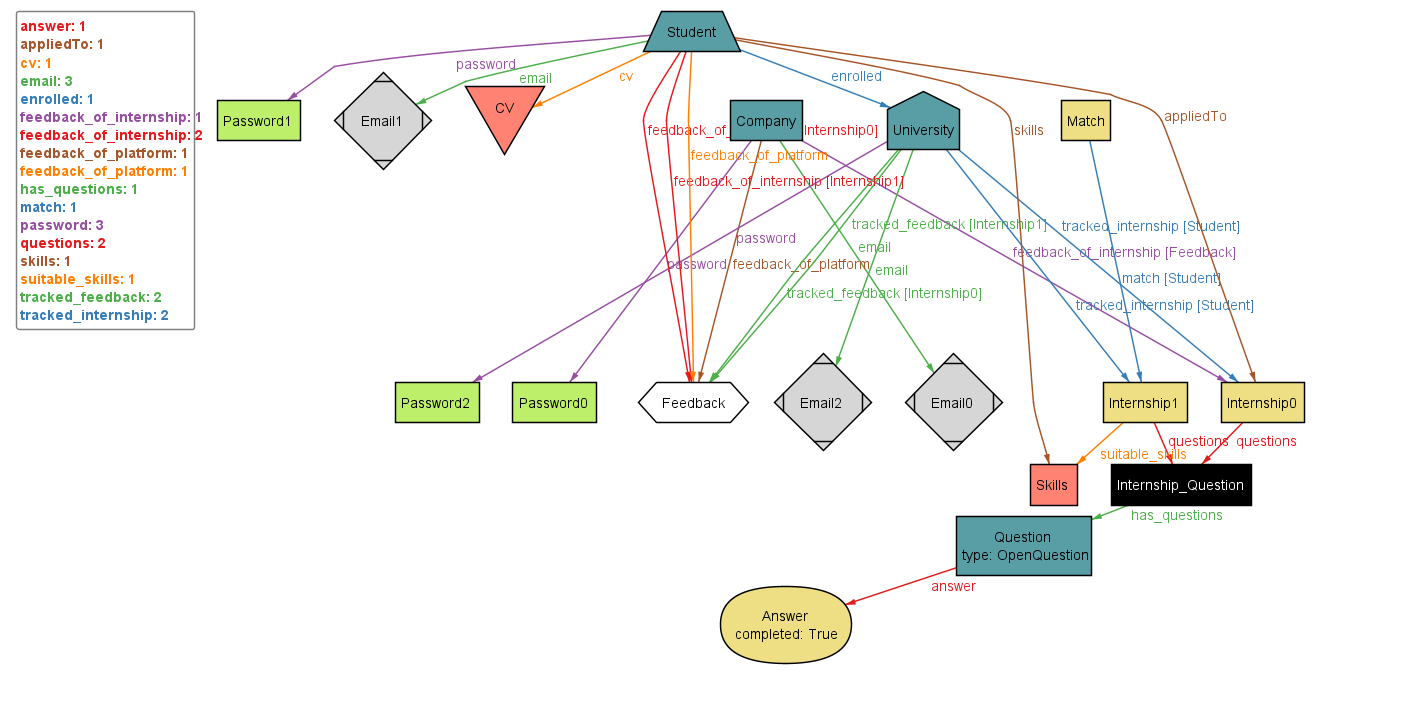
\includegraphics[angle=270, width=0.65\linewidth]{Images/ImagesRASD/AlloySimpleWorld.png}
    \caption{Simple world description in Alloy}
    \label{fig:simple-world}
\end{figure}



\pagebreak


\chapter{Effort Spent}
\section{Effort Spent}

\begin{table}[ht!]
\centering
\renewcommand{\arraystretch}{1.6}
\begin{tabular}{|c|l|c|}
\hline
\textbf{Member of Group} & \textbf{Effort Spent} & \textbf{Hours} \\ \hline
\multirow{5}{*}{Giovanni Vaccarino} 
    & Introduction & 2h \\ \cline{2-3}
    & Overall Description & 1h \\ \cline{2-3}
    & Specific Requirements & 3h \\ \cline{2-3}
    & Formal Analysis & 1h \\ \hline
\multirow{5}{*}{Vittorio Palladino} 
    & Introduction & 2h \\ \cline{2-3}
    & Overall Description & 1h \\ \cline{2-3}
    & Specific Requirements & 1h \\ \cline{2-3}
    & Formal Analysis & 4h \\ \hline
\multirow{5}{*}{Nicolò Vacis} 
    & Introduction & 1h \\ \cline{2-3}
    & Overall Description & 3h \\ \cline{2-3}
    & Specific Requirements & 2h \\ \cline{2-3}
    & Formal Analysis & 1h \\ \hline
\end{tabular}
\caption{Effort spent by each member of the group}
\end{table}


\chapter{References}
\section{References}
\begin{itemize}
    \item 2024-2025 Software Engineering 2 - Assignment RASD
\end{itemize}


\cleardoublepage

\end{document}
